\documentclass{article}
\usepackage{graphicx}
\usepackage{hyperref}
\usepackage{amsmath}
\usepackage[a4paper, total={6in, 8in}]{geometry}

\begin{document}

\begin{titlepage}
    \begin{center}
        \vspace*{1cm}
            
        \Huge
        \textbf{Electricity Usage Optimizer}
            
        \vspace{0.5cm}
        \LARGE
        Miniproject Report
        
        \date{today}
            
        \vspace{1.5cm}
            
        Pontus Hedlund, Sanna Korpi, Topi Ranta
            
        \vfill
            

            
        \vspace{0.8cm}
            
            
        \Large
        University of Helsinki\\
        Introduction to Data Science\\
        31.10.2022\\
            
    \end{center}
\end{titlepage}

\tableofcontents

\vspace{30.0 cm}

\section{A Simple Prediction of Electricity Price Development}
\label{section:introduction}

This report describes technical aspects of an electricity price prediction software made as Introduction to Data Science course mini project. The estimation tool is a Python web application that provides a 36-hour electricity price development prediction. The forecast is shown as an hourly three-step recommendation scale and it is based on a linear regression model trained with historical data including electricity price, power consumption and weather data.

The report includes references to \href{https://github.com/IDS-mini/electricity}{the project repository in Github}. In addition to the data exploration, the regression model and the web application source code, the repository also includes our \href{https://github.com/IDS-mini/electricity/blob/main/marketing/Mini-Project-Canvas-Hedlund-Korpi-Ranta.pdf}{project canvas}, \href{https://github.com/IDS-mini/electricity/blob/main/marketing/presentation.pptx}{product pitch presentation} and \href{https://github.com/IDS-mini/electricity/blob/main/src/app/templates/index.html}{web application home page}. As this report does not discuss the added value or the business side of the project, it is advisable to walk through those documents before reading this technical report.

The rest of the report is composed as follows: the data used and data preprocessing is described in Chapter \ref{section:data}. The prediction formulation and the linear regression model used in the project are presented in Chapter \ref{section:analysis}. User experience and results delivery for the end user are reported in Chapter \ref{section:delivery}.

\section{Data}
\label{section:data}

In order to produce the prediction, several sets of historical data were used. The data sets are described in Subchapter \ref{subsection:datadescription} and comments on the data exploration and preprocessing in Subchapter \ref{subsection:eda}. Data storaging and protection are reported in Subchapter \ref{subsection:warehousing}.

\subsection{Data Used in the Project}
\label{subsection:datadescription}

The data sources used in the project are \href{https://data.fingrid.fi/en}{Fingrid Wind Power Production and Total Consumption Data}, \href{https://transparency.entsoe.eu}{Entsoe Day-ahead Market Price Data}, \href{https://en.ilmatieteenlaitos.fi/open-data}{Finnish Meteorological Institute Weather Observation Data for Kumpula, Helsinki}. The data was accessed in two ways. Large, historical data sets were manually downloaded for exploration, feature extraction and model training and programmatic access was used to enable the web application to get the latest data for user predictions. The programmatic access includes API connections and web scraping.

Even though all the data is available for free, some sources require registering an account to download the full data or access most recent data via API. Characteristics of the data sources are presented in Table \ref{table:source-characteristics}.

\begin{table}[b] 
\centering 
\begin{tabular}{l||l c c} 
data set & Format & Access via & Registration\\ 
\hline \hline
Entsoe & CSV & UIM, WS  & Required for full history access \\
FMI & CSV & UI, API & Not required \\
Fingrid & CSV & UIM, API & Required for API access \\
\hline
\end{tabular}
\caption{The data sources used in the project. UIM is abbreviation for manual download via user interface and WS for web scraping.}
\label{table:source-characteristics}
\end{table}

Entsoe Day-ahead Prices data consists of hourly electricity market prices for Finnish Bidding Zone that covers the whole country. \href{https://data.fingrid.fi/en/data set/wind-power-generation}{The Wind Power Production} data set includes hourly wind power production in Finland in $MWh/h$, \href{https://data.fingrid.fi/en/data set/electricity-consumption-in-finland}{Electricity Consumption} data set $MWh/h$ consumption and from \href{https://en.ilmatieteenlaitos.fi/open-data}{Weather Data} we picked air pressure, rain, humidity, temperature and wind. \href{https://www.helen.fi/en/company/responsibility/current-topics/open-data}{Helen District Heating Power Data} was investigated but was reject, as the data was only available until the end of year 2021.

All the data used in project is provided in one hour interval thus making data integration rather easy. The historical data was downloaded spanning from the beginning of 2019 as far ahead as possible.

\subsection{Exploratory Data Analysis and Data Preprocessing}
\label{subsection:eda}

The purpose of the exploratory data analysis (EDA) and data preprocessing phase was to understand the data and its possible shortages and produce an integrated data set for model training with missing values imputed. This phase was conducted in series of Jupyter Notebook files. The cleaned csv files were written into Apache Parquet format for better data compression and reading performance before integration.

\begin{table}[b] 
\centering 
\begin{tabular}{l||l c} 
Data set & Imputation method & File\\ 
\hline \hline
Day-ahead & Previous neighbor & \href{https://github.com/IDS-mini/electricity/blob/main/data/day-ahead_eda.ipynb}{day-ahead\_eda.ipynb}\\
Consumption & - & \href{https://github.com/IDS-mini/electricity/blob/main/data/consumption_eda.ipynb}{consumption\_eda.ipynb} \\
Weather & Neighbor values mean & \href{https://github.com/IDS-mini/electricity/blob/main/data/weather_eda.ipynb}{weather\_eda.ipynb} \\
Wind power & - & \href{https://github.com/IDS-mini/electricity/blob/main/data/wind_power_eda.ipynb}{wind\_power\_eda.ipynb}\\
\hline
\end{tabular}
\caption{The data sets used to train the model. Link to data sets EDA Jupyter notebook file is presented in the File column.}
\label{table:eda}
\end{table}

We created Jupyter Notebooks for all data sources to clean and process the data.
The products of this process was data sets with the datetime field as index.
Two separate data sets were created for each data source - historical and a time series forecast.
The historical data is used for training the model, and the forecast combined with available amendments from APIs to construct the final predicted price.

\subsection{Data Warehousing and Data Protection}
\label{subsection:warehousing}

All data used for our purpose is publicly available. No data subject to the GDPR act is used, since we are not collecting any data for individuals.

\section{Data Analysis}
\label{section:analysis}

%% target value
\subsection{Feature Extraction}
\label{subsection:extraction}

Features extracted for the model were:

'WindMWh', 'ConsumptionMWh', 'pressure', 'rain', 'humidity',

'temperature', 'wind' and the target value was 'price'.


\subsection{Gathering the Data for the Prediction}
\label{subsection:datafilling}

Since the model is trained on past data, all the same variables need to be present when performing the prediction. Since all of these are not available for the prediction time, we created time series forecasts that should give a best estimate of the values (See figure \ref{fig:consumption}).

\begin{figure}
    \centering
    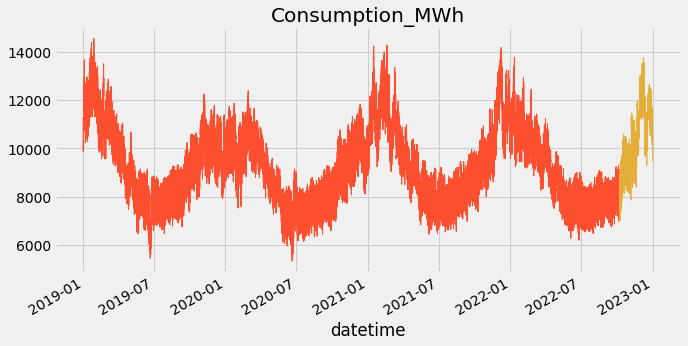
\includegraphics[width=15cm]{report/images/consumption.png}
    \caption{Time series for Consumption in MWh with historical data in red and the forecast in orange.}
    \label{fig:consumption}
\end{figure}

\subsection{Time Series Prediction with XGBoost}
\label{subsection:xgboost}

The ML model used for this application is the XGBoost Regressor, which is an ensemble method based on gradient-boosted decision trees. It was found to be very fast to train and very accurate.

When training the forecasts, we used cross validation with time series splits (See figure \ref{fig:ts-cross-validation}).

\begin{figure}
    \centering
    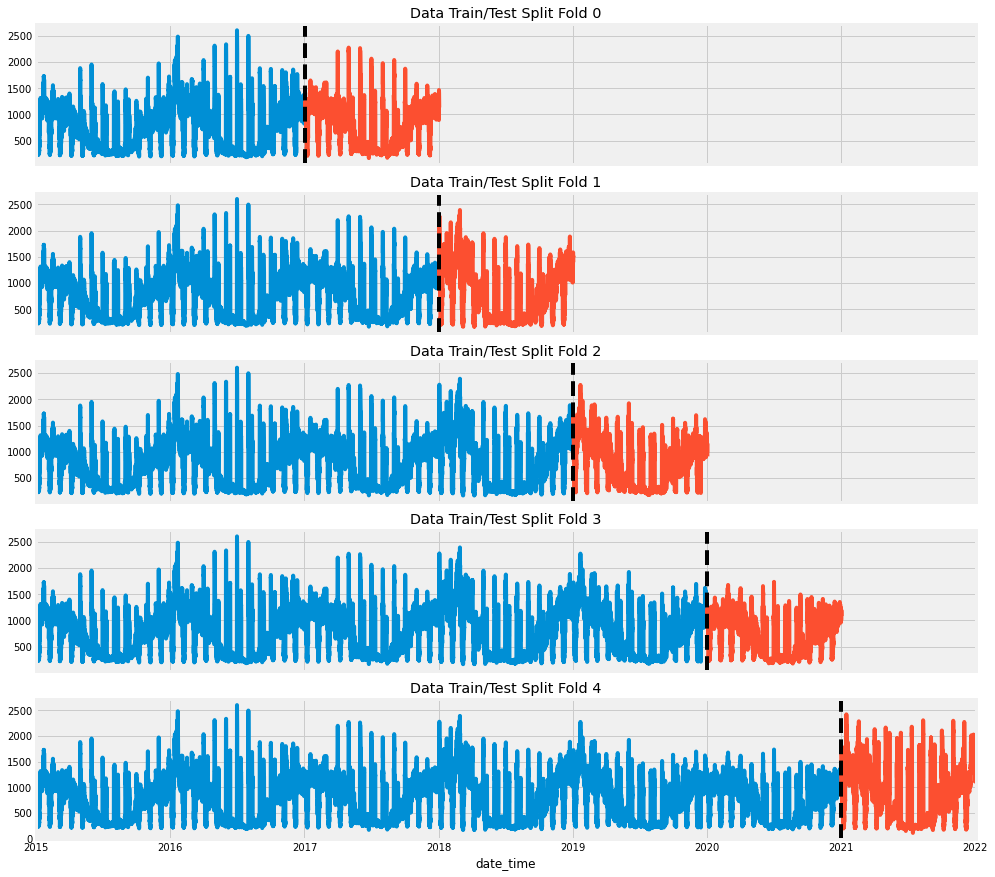
\includegraphics[width=15cm]{report/images/ts-cross-validation.png}
    \caption{Cross validation using Time Series Splits with each split being a year.}
    \label{fig:ts-cross-validation}
\end{figure}



\section{Delivering Results for the End User}
\label{section:delivery}

We calculate a simple moving average (SMA) of the electricity price with a window of 168 hours (7 days) to create a reference price point. For each prediction time, we compare the predicted or known price to the index via equation \ref{eq:index}.


\begin{equation} \label{eq:index}
\text{"Price Index"}_i = \frac{\text{SMA}_i}{\text{"Predicted Price"}_i}
\end{equation}

The price index is then classified as follows:

\begin{enumerate}
    \item $\text{"Price Index"}_i < 0.8$ : "Boost"
    \item $0.8 \leq \text{"Price Index"}_i \leq 1.2$ : "Maintain"
    \item $\text{"Price Index"}_i > 1.2$ : "Restrict"
\end{enumerate}

\subsection{Web Application}
\label{subsection:server}

Our deliverable is a web application built with FastAPI that serves a landing page and a page for planning. The plan page shows a table with hourly times for the next 36 hours with a recommendation and the price index. The whole package is available on Github at https://github.com/IDS-mini/electricity .

\subsection{Visualization and User Experience}
\label{subsection:ux}

%% no gdpr data gathered from the user either

\section{Conclusions}
\label{section:conclusions}

%% what was achieved
%% what was learned
%% what we would do differently
%% ideas for further development or research


\end{document}

